\documentclass[english, 11 pt, class=article, crop=false]{standalone}
%\documentclass[english, 11 pt]{report}
\usepackage[T1]{fontenc}
\usepackage[utf8]{luainputenc}
\usepackage{babel}
\usepackage[hidelinks, bookmarks]{hyperref}
\usepackage{geometry}
\geometry{verbose,tmargin=1cm,bmargin=3cm,lmargin=4cm,rmargin=4cm,headheight=3cm,headsep=1cm,footskip=1cm}
\setlength{\parindent}{0bp}
\usepackage{amsmath}
\usepackage{amssymb}
\usepackage{esint}
\usepackage{import}
\usepackage[subpreambles=false]{standalone}
%\makeatletter
\addto\captionsenglish{\renewcommand{\chaptername}{Kapittel}}
\makeatother
\usepackage{tocloft}
\addto\captionsenglish{\renewcommand{\contentsname}{Innhold}}
\usepackage{graphicx}
\usepackage{placeins}
\raggedbottom
\usepackage{calc}
\usepackage{cancel}
\makeatletter
\usepackage{color}
\definecolor{shadecolor}{rgb}{0.105469, 0.613281, 1}
\usepackage{framed}
\usepackage{wrapfig}
\usepackage{bm}
\usepackage{ntheorem}

\usepackage{ragged2e}
\RaggedRight
\raggedbottom
\frenchspacing

\newcounter{lign}[section]
\newenvironment{lign}[1][]{\Large \refstepcounter{lign} \large
	\textbf{\thelign #1} \rmfamily}{\par\medskip}
\numberwithin{lign}{section}
\numberwithin{equation}{section}
\usepackage{xcolor}
\usepackage{icomma}
\usepackage{mathtools}
\usepackage{lmodern} % load a font with all the characters
\usepackage{xr-hyper}
\makeatother
\usepackage[many]{tcolorbox}

%\setlength{\parskip}{\medskipamount}
\newcommand{\parskiplength}{11pt}
%\setlength{\parskip}{0 pt}
\newcommand\eks[2][]{\begin{tcolorbox}[enhanced jigsaw,boxrule=0.3 mm, arc=0mm,breakable,colback=green!30] {\large \textbf{Eksempel #1} \vspace{\parskiplength}\\} #2 \vspace{1pt} \end{tcolorbox}\vspace{1pt}}

\newcommand\fref[2][]{\hyperref[#2]{\textsl{Figur \ref*{#2}#1}}}
\newcommand{\hr}[2]{\hyperref[#2]{\color{blue}\textsl{#1}}}

\newcommand\rgg[2][]{\begin{tcolorbox}[boxrule=0.3 mm, arc=0mm,colback=orange!55] #2 \vspace{1pt} \end{tcolorbox}\vspace{-2pt}}
\newcommand\alg[1]{\begin{align*} #1 \end{align*}}
\newcommand\algv[1]{\vspace{-11 pt} \begin{align*} #1 \end{align*}}
\newcommand\vs{\vspace{-11 pt}}
\newcommand\g[1]{\begin{center} {\tt #1}  \end{center}}
\newcommand\gv[1]{\begin{center} \vspace{-22 pt} {\tt #1} \vspace{-11 pt} \end{center}}
%\addto\captionsenglish{\renewcommand{\contentsname}{Løsningsforslag tentamen R2 H2015}}

% Farger
\colorlet{shadecolor}{blue!30} 

% Figur
\usepackage{float}
\usepackage{subfig}
\captionsetup[subfigure]{labelformat=empty}
\usepackage{esvect}

\newcommand\sv{\textbf{Svar:} \vspace{5 pt} \\}

%Tableofconents
\renewcommand{\cfttoctitlefont}{\Large\bfseries}
\setlength{\cftsubsecindent}{2 cm}
\newcommand\tocskip{6 pt}
\setlength{\cftaftertoctitleskip}{30 pt}
\setlength{\cftbeforesecskip}{\tocskip}
%\setlength{\cftbeforesubsecskip}{\tocskip}

%Footnote:
\usepackage[bottom, hang, flushmargin]{footmisc}
\usepackage{perpage} 
\MakePerPage{footnote}
\addtolength{\footnotesep}{2mm}
\renewcommand{\thefootnote}{\arabic{footnote}}
\renewcommand\footnoterule{\rule{\linewidth}{0.4pt}}

%asin, atan, acos
\DeclareMathOperator{\atan}{atan}
\DeclareMathOperator{\acos}{acos}
\DeclareMathOperator{\asin}{asin}

%Tabell
\addto\captionsenglish{\renewcommand{\tablename}{Figur}}

% Figur
\usepackage[font=footnotesize,labelfont=sl]{caption}
\addto\captionsenglish{\renewcommand{\figurename}{Figur}}

% Figurer
\newcommand\scr[1]{/home/sindre/R/scr/#1}
\newcommand\asym[1]{/home/sindre/R/asymptote/#1}

%Toc for seksjoner
\newcommand\tsec[1]{\phantomsection\addcontentsline{toc}{section}{#1}
	\section*{#1}}
%\newcommand\tssec[1]{\subsection*{#1}\addcontentsline{toc}{subsection}{#1}}
\newcommand\tssec[1]{\subsection*{#1}}
% GeoGebra
\newcommand{\cms}[2]{{\tt #1( #2 )}}
\newcommand{\cm}[2]{{\large \tt #1( #2 )} \gvs \\}
\newcommand{\cmc}[2]{{\large \tt #1( #2 )} \large (CAS)  \gvs \\ \normalsize}
\newcommand{\cmk}[2]{{\large \tt #1( #2 )} \large (Inntastingsfelt)  \gvs \\ \normalsize}

\newcommand\gvs{\vspace{11 pt}}

\newcommand\vsk{\vspace{11 pt}}
\newcommand{\merk}{\vsk \textsl{Merk}: }
\newcommand{\fig}[1]{
\begin{figure}
	\centering
	\includegraphics[scale=0.5]{fig/#1}
\end{figure}
}
\newcommand{\figc}[1]{
		\centering
		\includegraphics[scale=0.5]{fig/#1}
}

% Opg
%\newcommand{\opgt}{\phantomsection \addcontentsline{toc}{section}{Oppgaver} \section*{Oppgaver for kapittel \thechapter}}
\newcounter{opg}
\numberwithin{opg}{section}

\newcommand{\opl}[1]{\vspace{15pt} \refstepcounter{opg} \textbf{\theopg} \vspace{2 pt} \label{#1} \\}



\begin{document}
\eqlen
\opgt
\setcounter{section}{1}	

\opl{odpar}
\textbf{a)} Skriv opp de tre første partallene. Lag en rekursiv og en eksplisitt formel for det $ i $-te partallet.\os
	
\textbf{b)} Skriv opp de tre første oddetallene. Lag en eksplisitt formel for det $ i $-te oddetallet. 

\opl{eksar}
Finn det eksplisitte uttrykket til  den aritmetiske følgen når du vet at\os
\begin{tabular}{@{}l l}	
	\textbf{a)} $ a_1=3 $ og $ a_4 = 30 $ \os 
	\textbf{b)} $ a_1 = 5 $ og $ a_{11} = -25 $ \os
	\textbf{c)} $ a_3 =14 $ og $ a_5=26 $ 
\end{tabular}\os

\opl{eksgeo}
Finn det eksplisitte uttrykket til den geometriske følgen når du vet at\os
\begin{tabular}{@{}l l}	
	\textbf{a)} $ a_1=\frac{1}{2} $ og $ a_2 = \frac{1}{6} $ \os 
	\textbf{b)} $ a_1 = 5 $ og $ a_4 = 40 $
\end{tabular} \os

\begin{comment}
	\op
Bruk formelen fra oppgave \textsl{\ref{sumkvad}a} og det eksplisitte uttrykket for en aritmetisk følge til å forklare at summen av en aritmetisk rekke kan skrives som:
\[na_1 +\frac{dn(n-1)}{2} \]


\op
a) Bruk (\ref{sumg}) og vis at summen $ S_\infty $ når $ n\to\infty $ blir:
\[ S_\infty=a_1\frac{1}{1-k} \]
for $ |k|<1 $.
\end{comment}
\nes

\opl{parodd}
\textbf{a)} Bruk figuren under til å forklare at summen $ S_n $ av de $ n $ første naturlige tallene er gitt ved
\[S_n=\frac{n(n+1)}{2}  \]

\begin{figure}
	\centering
	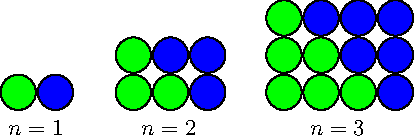
\includegraphics[]{../../asymptote/sum}
\end{figure}\vs
\textbf{b)} Skriv opp summen av det første, de to første og de tre første  oddetallene. Bruk en lignende figur som i oppgave a) til å vise at summen $ S_n $ av de $ n $ første oddetallene er
\[ S_n = n^2 \] 

\opl{sum10ar}
Finn $ S_{10} $ for rekkene:\os
\begin{tabular}{@{}l l}	
	\textbf{a)} $ 7+13+19+25+\ldots $\quad
	\textbf{b)} $ 1+9+17+25+\ldots $
\end{tabular} \os

\opl{ar435}
Gitt rekken 
\[ 8+11+14+\ldots \]
For hvilken $ n $ er summen av rekken lik 435?

\opl{viseks3}
Bruk summen av en aritmetisk rekke til å vise at ligningen gitt i \hyperref[prodind]{\textsl{Eksempel 3}} på s. \pageref{prodind} er sann.

\opl{geon}
Gitt rekken
\[ 3+12+48+\ldots+768 \]
Finn summen av rekken. 

\opl{geoa12}
En geometrisk rekke har $ {a_1 = 2} $ og $ {k=3} $.\os 

\textbf{a)} Vis at summen $ S_n $ kan skrives som:
\[ S_n = 3^n-1 \]
\textbf{b)} Regn ut summen for de tre første leddene.\os

\textbf{c)} For hvilken $ n $ er $ S_n=728 $?

\opl{geospar}
Du ønsker å spare penger i en bank som gir 2\,\% månedlig rente. Du sparer ved å foreta et innskudd den 1. i hver måned, og du starter 01.01.2017.\os

\textbf{a)} Skriv rekken som viser hvor mye penger du har i banken 01.05.2017. Innskuddet 01.05 skal tas med.\os

\textbf{b)} Sett opp et uttrykk $ P(n) $ som viser hvor mye penger du har i banken $ n $ måneder etter 01.01.2017, medregnet innskuddet samme måned.

\begin{comment}
\textbf{c)} Hvis du fortsetter å spare slik, og medregner innskudd samme måned, når vil du ha 24200 kr på konto? 
\end{comment}

\opl{1over4}
Gitt den uendelige rekken
\[ 4+1+\frac{1}{4}+\ldots \]
\textbf{a)} Forklar hvorfor rekken er konvergent.\os

\textbf{b)} Finn summen av den uendelige rekken.

\begin{comment}
	\opl{stav} 
	Tenk at uendelig mange personer skal sette sammen en stav. Første person legger på en meter, neste person legger på 0.1 m, neste legger på 0.01 m osv. Hvor lang blir staven?
\end{comment}
\newpage
\opl{099er1}
\textbf{a)} Skriv det uendelige desimaltallet 0.999... som en uendelig geometrisk rekke.\os

\textbf{b)} Forklar hvorfor rekken er konvergent og bruk dette faktumet til å finne summen av rekken. 

\opl{geokonv}
Gitt den uendelige rekken
\[\frac{1}{3} +\frac{1}{3}(x-2)+ \frac{1}{3}(x-2)^2+\ldots\]
\textbf{a)} For hvilke $ x $ er rekken konvergent? \os

\textbf{b)} For hvilken $ x $ er $ S_n = \frac{2}{9} $?\os

\textbf{c)} For hvilken $ x $ er $ S_n= \frac{1}{6}$? \os

\nes
\opl{ind}
Vis ved induksjon at for alle $ n\in \mathbb{N} $ er\\[10pt]
\begin{tabular}{@{}l l}	
	\textbf{a)} $ 1+2+3+\ldots+n = \dfrac{n(n+1)}{2} $ \\[10pt]
	\textbf{b)} $ 1+2 +2^2 +\ldots+ 2^{n-1}= 2^n-1$\\[10pt]
	\textbf{c)} $ 4+4^2+4^3+\ldots+4^n = \dfrac{4}{3}(4^n-1) $ \\[10pt]
	\textbf{d)} $ 1^2 + 2^2+3^2+ \ldots+ n^2 = \dfrac{n(2n+1)(n+1)}{6} $ 
\end{tabular} 

\opl{div3}
Vis ved induksjon at $ n(n^2+2) $ er delelig med 3 for alle $ n\in\mathbb{N} $.

\opl{factorials}
\textbf{a)}
Vis ved induksjon at:
\[\frac{1\cdot2}{1}\cdot\frac{1\cdot2\cdot3\cdot4}{1\cdot2\cdot3}\cdot
\ldots\cdot\frac{(2n)!}{(2n-1)!}=2^n n! \]
\textsl{Hint}: \y{(2(k+1))!=(2k+1)!(2k+2)}.\os

\textbf{b)} Hvordan kan venstresiden i a) skrives enklere? Utfør induksjonsbeviset på nytt etter forenklingen.
\newpage
\ekspop 
Målet med denne oppgaven er å, uten bruk av induksjon, vise at summen av $ n $ kvadrater er gitt ved følgende formel:
\[ \sum\limits_{i=1}^n i^2 = \frac{n(2n+1)(n+1)}{6} \tag{I}\label{sumkvad}\]
\textbf{a)} Forklar hvorfor vi kan skrive
\[ 1^2 + 2^2 + 3^2+\ldots = 1 + (1+3) + (1+3+5)+ \ldots  \]
\textsl{Hint}: se opg. \ref{parodd} b).\os

\textbf{b)} Ut ifra det du fant i a), forklar at
\[ \sum\limits_{i=1}^n i^2 = n+\sum\limits_{i=1}^n (n-i)(2i+1)  \]
\textbf{c)} Skriv ut alle kjente summer fra b) og løs ligningen med hensyn på $ \sum\limits_{i=1}^n i^2 $, du skal da komme fram til (\ref{sumkvad}).
\end{document}
\begin{comment}
\opl{eksplar}
Finn det eksplisitte uttrykket til den aritmetiske rekken når du vet at:
\os
\begin{tabular}{@{}l l}	
\textbf{a)} $ a_1=-5 $ og $ a_8=44 $. \os 
\textbf{b)} $ a_7=39 $ og $ d=6 $. \os
\textbf{c)} $ a_5 = 16 $ og $ a_{10} = 31 $
\end{tabular}
\end{comment}